\chapter{Interaksi berkas}
\section{Pendahuluan}
Lingkup interaksi di sini adalah interaksi dengan berkas teks (\texttt{ASCII}) untuk tujuan membaca, memformat ulang dalam bentuk penyajian di layar maupun disimpan kembali ke berkas teks. Selain teks, maka diperlukan proses tambahan untuk mengubahnya. Hal ini disebabkan karena umumnya data yang dianalisis dalam keilmuan data disimpan dalam bentuk teks dengan format csv (\textit{comma separated value}). Beberapa mungkin disimpan dalam aplikasi \textit{spreadsheet} seperti Microsoft Excel$\copyright$. 

Selain itu, kita mungkin saja terlibat dengan lebih dari satu berkas yang tersebar di \textit{sub directory}  yang berbeda. Atau bisa saja perlu menyusun ulang struktur \textit{directory} baru yang lebih mudah dipahami. Satu contoh kasus\footnote{\url{http://otmedia.lirmm.fr/LifeCLEF/PlantCLEF2017/}}, data yang berisi citra tumbuhan dari bagian yang berbeda seperti bunga, daun atau buah tidak tersusun berdasarkan bagian-bagian tersebut. Sementara kita memerlukan data tersebut tersusun berdasarkan bagian tumbuhan, bahkan mengikuti struktur \textit{family-genus-species} sehingga diperlukan \lstlistingname~\ref{lst:pynonxmlreader}. Atau contoh lain\footnote{\url{https://www.unsw.adfa.edu.au/unsw-canberra-cyber/cybersecurity/ADFA-NB15-Datasets/bot\_iot.php}}, di mana dataset terpisah dalam berkas yang berbeda untuk kemudahan proses unduh. Sementara di masing-masing berkas terdapat data dari kelas-kelas yang berbeda. Untuk mengetahui proporsi data dari setiap kelas, kita perlu membaca semua potongan berkas yang tersedia.

\scriptsize
\lstinputlisting[language=python, numbers=left, numberstyle=\tiny, caption=Mengubah pengelompokan data berdasarkan bagian tumbuhan, showstringspaces=false, label=lst:pynonxmlreader]{script/pynonxmlreader.py}
\normalsize

\section{Berkas tunggal}
Sebagai bahan latihan, kita akan membaca dataset iris\footnote{\url{https://archive.ics.uci.edu/ml/machine-learning-databases/iris/iris.data}}. Pembacaan dilakukan baris per baris dan menampilkan isinnya. Dataset tersebut berisi informasi tentang dimensi bunga iris, yaitu \textit{sepal length}, \textit{sepal width}, \textit{petal length}, \textit{petal width} yang masing-masing dalam satuan \texttt{cm}. Kolom terakhir merupakan kelas dari 3 jenis bunga iris yang ada pada dataset tersebut, masing-masing Setosa, Versicolor dan Virginica. Data yang ditampilkan harus memiliki format 5 baris yang setiap barisnya adalah

\texttt{jenis bunga iris ke-i:}

\texttt{sepal length = $\ldots$ cm}

\texttt{sepal width = $\ldots$ cm}

\texttt{petal length = $\ldots$ cm}

\texttt{petal width = $\ldots$ cm}


Perhatikan \lstlistingname~\ref{lst:bacairis}. Program tersebut bertujuan untuk membaca data yang disimpan dalam bentuk tabular dan menampilkannya di layar dengan format baru. Simpan \lstlistingname~\ref{lst:bacairis} dalam berkas berekstensi \texttt{.py} lalu jalankan untuk melihat hasilnya dengan perintah \texttt{python nama\_file.py}.

\lstinputlisting[language=python, numbers=left, numberstyle=\small, caption=Membaca dataset iris dan menampilkan isinya dengan format tertentu, showstringspaces=false, label=lst:bacairis]{script/bacairis.py}

Berikut adalah penjelasan perintah pada \lstlistingname~\ref{lst:bacairis} berdasarkan urutan barisnya.
\begin{enumerate}
  \item Baris ke-1: membuat \texttt{pointer} ke berkas, yang dalam contoh ini adalah \texttt{iris.data} yang menjadi argumen pertama dari fungsi \texttt{open}. Sedangkan argumen keduanya adalah \texttt{'r'}, menunjukkan mode baca. Untuk mode tulis, gunakan argumen \texttt{'w'}.
  \item Baris ke-2: menyiapkan variabel \textit{dictionary} yang akan digunakan untuk menyimpan informasi kelas data berikut jumlahnya.
  \item Baris ke-3: menyiapkan variabel \texttt{int} yang akan digunakan untuk menyimpan informasi total data.
  \item Baris ke-4: memulai perulangan untuk membaca berkas per baris melalui perintah \texttt{a.readlines()}. Jika hanya diperlukan untuk membaca satu baris saja, gunakan perintah \texttt{a.readline()}. Baris yang berhasil dibaca akan disimpan dalam variabel \texttt{baris}.
  \item Baris ke-5 \& 18: penanganan kesalahan yang disebabkan oleh kondisi berkas yang baris terakhirnya kosong sehingga tidak dapat diolah seperti baris lain di atasnya.
  \item Baris ke-6: memisahkan baris yang dibaca berdasarkan pembatas (\textit{delimiter}) berupa karakter '\texttt{,}'. Hasilnya disimpan dalam \texttt{list} dengan nama \texttt{element}.
  \item Baris ke-7: membersihkan \texttt{element} terakhir dari karakter \escape{n}, dan menyimpannya dalan \texttt{list} dengan nama \texttt{kelas}. Nilai dari \texttt{kelas} yang akan digunakan disimpan di \texttt{kelas[0]}.
  \item Baris ke-8 s/d 11: blok kondisi yang ketika nilai kelas belum ada di variabel \texttt{jenis}, ia akan ditambahkan sebagai \texttt{key} dengan nilai \texttt{1}. Sedangkan jika sudah menjadi salah satu \texttt{key}, maka nilainya ditambah \texttt{1}.
  \item Baris ke-12 s/d 16: menampilkan isi dari baris yang sedang dibaca, yang sebelumnya telah dipisah-pisah ke layar. Sejatinya, perintah \texttt{print} menerima argumen \texttt{str}. Jika ada karakter/kata eksplisit akan ditampilkan bersama karakter/kata yang disimpan pada variabel, maka penulisannya perlu dibedakan, dan dihubungkan dengan operator \texttt{+}. Dari sini terlihat bahwa operator \texttt{+} tidak hanya dapat digunakan dalam operasi aritmatika. Khusus untuk variabel yang akan ditampilkan dengan perintah \texttt{print}, tetapi belum dalam bentuk \texttt{str} (seperti pada baris ke-12), maka perlu dilakukan transformasi. Perintah yang digunakan adalah \texttt{str}, sebagai target jenis variabel yang diperlukan. Jika pada kondisi tertentu, diperlukan untuk mengubah jenis variabel ke \texttt{int}, maka digunakan perintah yang sama dengan target jenis variabelnya, dalam hal ini \texttt{int}.
  \item Baris ke-17: mengakumulasi total data dari berkas yang dibaca.
  \item Baris ke-19: mendefinisikan perintah ketika baris yang dibaca tidak dapat diolah dengan perintah yang sama dengan baris lain.
  \item Baris ke-20: menghapus \texttt{pointer} ke berkas yang telah selesai digunakan.
  \item Baris ke-21: mencetak informasi
  \item Baris ke-22 \& 23: mencetak informasi statistik (jumlah data per kelas dan proporsinya dalam \%). Baris ke-22 digunakan untuk membuat perulangan berdasarkan jumlah kelas yang dalam contoh ini adalah jumlah elem dari variabel \texttt{jenis}. Sedangkan baris ke-23 digunakan untuk mencetak informasi berikut:
  \begin{itemize}
     \item nama kelas yang direpresentasikan melalui variabel \texttt{i}.
     \item jumlah data untuk kelas tertentu yang direpresentasikan melalui variabel \texttt{jenis[i]}. Karena jenisnya \texttt{int}, maka perlu diubah ke \texttt{str}.
     \item proporsi jumlah data, dilakukan dengan cara melakukan operasi pembagian jumlah data per kelas terhadap total data. Hasilnya ditampilkan dengan format dua angka desimal (\texttt{:4.2f}).
   \end{itemize} 
   Hasil dari menampilkan informasi statistik tersebut ditampilkan di \figurename~\ref{fig:iristat}.
\end{enumerate}

\begin{figure}
  \begin{center}
    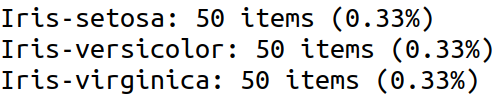
\includegraphics[scale=2]{pics/iristat.png}
    \caption{Informasi statistik dataset iris}
    \label{fig:iristat}
  \end{center}
\end{figure}

\section{Berkas jamak}
Selanjutnya, sebagai latihan kedua, dataset yang akan digunakan adalah dataset tentang keamanan siber\footnote{\url{https://www.unsw.adfa.edu.au/unsw-canberra-cyber/cybersecurity/ADFA-NB15-Datasets/bot\_iot.php}}. Untuk seluruh dataset, terdapat 74 berkas yang berbeda. Tetapi, berkas pertamanya kosong sehingga akan diabakan dalam pembacaan. Perhatikan \lstlistingname~\ref{lst:catexplore}.

\lstinputlisting[language=python, numbers=left, numberstyle=\small, caption=Menghitung total data untuk setiap kelas, showstringspaces=false, label=lst:catexplore]{script/categoryExplore.py}

\section{Modifikasi dataset}
Yang dimaksud dengan modifikasi di sini adalah memilih bagian yang menarik untuk dianalisis. Sebagai contoh, salah satu dataset tentang keamanan siber\footnote{https://github.com/aawaskita/Cyber-Security-dataset/} memiliki fitur yang dapat dibagi menjadi beberapa kelompok. \lstlistingname~\ref{lst:featbased} mengilustrasikan bagaimana memisahkan data berdasarkan kelompok fitur tersebut. Kita bisa saja melakukan kajian tentang efektivitas penggunaan kelompok fitur yang berbeda terhadap akurasi suatu \textit{classifier}. Untuk dapat diklasifikasi, kolom kelas tetap disimpan di dataset untuk kelompok fitur berbeda.

\lstinputlisting[language=python, numbers=left, numberstyle=\small, caption=Memisahkan dataset ke dalam kelompok fitur yang berbeda, showstringspaces=false, label=lst:featbased]{script/featureBasedAttack.py}

Penjelasan baris-baris perintah dari \lstlistingname~\ref{lst:featbased} adalah sebagai berikut.
\begin{enumerate}
  \item Baris ke-1 s/d 6: membuat \texttt{pointer} ke berkas sumber (baris ke-1) maupun berkas target (baris ke-2 s/d 6). Kelompok fitur yang dimaksud masing-masing adalah diwakili oleh \texttt{pointer} yang dibuat di baris ke-2 s/d 6.
  \item Baris ke-7 s/d 12: membuat penanda kolom di mana kelompok fitur diletakkan di berkas sumber. Sebagai contoh, fitur \textit{basic} disimpan di kolom 6 s/d 18. Maka, untuk mengambil data dari kelompok fitur \textit{basic}, gunakan data yang disimpan kolom 6 s/d 18.
  \item Baris ke-13: memulai perulangan untuk membaca berkas baris per baris.
  \item Baris ke-14: memisahkan baris yang dibaca berdasarkan pembatas (\textit{delimiter}) berupa karakter '\texttt{,}'. Hasilnya disimpan dalam \texttt{list} dengan nama \texttt{element}.
  \item Baris ke-15: menyimpan data kelas yang disimpan di lokasi terkahir dari \texttt{element}.
  \item Baris ke-16 s/d 21: mengambil data dari 5 kolom pertama sebagai data yang harus ada di setiap kelompk fitur.
  \item Baris ke-23 s/d 25: mengambil data untuk kelompok fitur \textit{basic} dan diakhiri dengan menyimpan kelas data di kolom terakhir. Fungsi yang sama berlaku untuk
  \begin{itemize}
     \item baris ke-27 s/d 29 (untuk kelompok fitur \textit{content}),
     \item baris ke-31 s/d 33 (untuk kelompok fitur \textit{time}),
     \item baris ke-35 s/d 37 (untuk kelompok fitur \textit{general})
     \item serta baris ke-39 s/d 41 (untuk kelompok fitur \textit{connection}).
   \end{itemize}
   \item Baris ke-43 s/d 48: menghapus \texttt{pointer} ke berkas yang telah digunakan.
\end{enumerate} 

\section{Latihan}
\begin{enumerate}
  \item Modifikasi \lstlistingname~\ref{lst:bacairis} agar dapat dijalankan tanpa perlu pengetahuan tentang jumlah kolom
  \item Dataset\footnote{\url{https://www.unsw.adfa.edu.au/unsw-canberra-cyber/cybersecurity/ADFA-NB15-Datasets/bot\_iot.php}} menyediakan informasi sub kelas. Sebagai contoh, kelas \texttt{UDP} memiliki sub kelas \texttt{Dos} dan \texttt{DDoS}. Sementara \lstlistingname~\ref{lst:catexplore} hanya menampilkan informasi jumlah data per kelas. Karena itu, modifikasi \lstlistingname~\ref{lst:catexplore} agar dapat secara otomatis menghitung jumlah data per kelas sekaligus per sub kelas dan menampilkannya di layar.
  \item Berdasarkan pengetahuan yang diperoleh dari \lstlistingname~\ref{lst:featbased}, bangun program sejenis yang mampu memisahkan data pada Latihan kedua yang hanya berisi data-data dari dua kelas terbesar. Pengetahuan tentang dua kelas terbesar diperoleh dari Latihan kedua.
  \item Dataset \textit{android malware}\footnote{\url{https://www.unb.ca/cic/datasets/android-adware.html}} (opsi alamat\footnote{http://223.25.97.91:8006/dataset/CICAndMal2017CVS/}) mengelompokan \textit{malware} dalam \textit{directory} tertentu berdasarkan kelas dan sub kelasnya. Untuk melakukan analisis, data dari berbagai kelas/sub kelas disatukan dalam data latih dan data uji. Satukan data yang tersebar di berbagai \textit{directory} tersebut ke dalam satu berkas baru dengan mempelajari \lstlistingname~\ref{lst:pynonxmlreader}.
\end{enumerate}
